\documentclass[12pt]{article}
\title{The Candyman Can Do More ! }
\author{林橋毅 111502563}
\usepackage[UTF8]{ctex}
\usepackage{graphicx} %插入图片的宏包
\usepackage{float} %设置图片浮动位置的宏包
\usepackage{caption}
\usepackage{subfigure} %插入多图时用子图显示的宏包
\usepackage{algorithm}
\usepackage{cite}
\usepackage{algpseudocode}
\usepackage{amsmath}
\usepackage{graphics}
\usepackage{epsfig}
\usepackage{amssymb}
\usepackage{bm}
\newtheorem{definition}{Definition}

\begin{document}
	\captionsetup[figure]{labelfont={bf}, labelformat={default}, labelsep=period,name={Fig.}}
	
	\maketitle
	
	\part{Introduction}
	本題是 UVA 10482 The candyman can 的加強版。將 $n$ 糖果分給 3 個人,第 $i$ 顆糖果的重量標示為 $w_i$,求得到最大糖果重量和跟最小糖果重量和的差最小是多少。也就是說要盡可能地公平的分糖果。
	原題目最多有 130 測資,每筆測資最多有 32 顆糖果,糖果重量為 0 至 20 克。但在加強版中,將糖果數量最大可以到 200 顆糖果,最重的糖果是 100 克,這將大大增加我們解題的困難度。 
	\part{Method}
	本節將會介紹我實作本題目的方法。
	\section{Botton-up Dynamic programming}
	使用 Botton-up 的解法,是原題目最好寫的寫法。\\
	
	首先,為了節省空間,我們只需要知道前兩個人分到的糖果重量就可以推算出第三人的糖果重量,因此我們需要計算所有糖果的總合,記做 $sum$。
	並且 $candies[i]$ 代表第 $i$ 顆糖果的重量。$dp[c1][c2]$ 作為 DP 陣列,紀錄當第一個人拿到糖果重量為 c1,第二個人為 c2 時,是否為合法的分配方法,如果是記為 $1$,反之為 $0$。\\
	
	$\left\{\begin{matrix}
		dp[c1+candies[i]][c2] = 1, if \ dp[c1][c2] == 1\\ 
		dp[c1][c2+candies[i]] = 1, if \ dp[c1][c2] == 1
	\end{matrix}\right.$\\ 

	有了所有的合法的解法,我們可以遍歷所有的解法,若該解法可行且比目前紀錄的最小值還小,我們就更新答案,將所有方法都檢查過後,我們可以得到最小的差,也就是答案了!
	
	\section{Bit operation}
	在上ㄧ節的基礎上,可以觀察到 $dp$ 陣列不是 0 就是 1,而且會根據 $dp[c1][c2]$ 決定值,但上ㄧ節的做法是一個一個慢慢做,但如果我能將 $dp$ 陣列的一個維度用 bitset 包裝起來,並且藉由 bitwise 運算能夠得到我們想要的結果,而且我們可以一口氣做很多個 bit,bit operation 在機器中是非常快且基本的運算,理論上我們應該能夠在上ㄧ節的基礎上提升好幾倍的運算速度。
	
	所以,我們可以將上節的兩個式子轉換成 bit operation 的形式,所以重新定義一個與 $dp$ 有同質關係的 bitset $bs$,同理 $bs[i][j]$($bs[i]$的第 $j$ 個 bit)即為 $dp[i][j]$。但不同的是 $bs[i]$ 是一組 bitset,所以我們可以對他做 bitwise operation,我將上節的式子轉換為 bitset 可用的操作關係式。
	 
	 	$\left\{\begin{matrix}
		 	bs[c1+candies[i]] = bs[c1+candies[i]] | bs[c1]\\ 
	 		bs[c1] = bs[c1] | (bs[c1] << candies[i])
		 \end{matrix}\right.$\\
	  
 	可見,相對上節公式的 $c2+candies[i]$ 其實就等價於向左 shift candies[i] 個 bit 在做 OR 運算。\\
 	
 	使用 bitset 可以幫助我們更輕易、直覺得寫出程式碼,也省去了自己撰寫 bitwise operation 的時間,而且能夠很有效的提升速度。
 	
 	\section{Top down}
 	使用 Top Down 的主要用意是只做需要做的內容就好,可以大幅加快 DP 的過程。
 	首先我們需要一個 check function,檢查使用前 $idx$ 個糖果能否組出最大值為 $M$ 最小值 $m$ 的分配方法,若能夠分配就為 1 反之為 0。
 	
 	我們的 $bs$ bitset,不再是與上節相同的定義了,此時定義 $bs[i][j]$ 為使用 i 顆糖果是否能組合出總重量為 j 的糖果,並且定義 $bs[0][0] = 1$,接著依序將 $bs$ 更新:當用 $i$ 顆糖果可以組合出 重量為 $j$ 的糖果時,那麼多一顆糖果,也就是 $i+1$ 時便可以組合出總重量為 $j+candies[i]$ 的糖果,我們可以簡單地得到式子:\\
 	
 	$
 	bs[i+1] = bs[i] | (bs[i] << candies[i])\\
 	$
 	
 	有了 bs 後,我們就可以可以知道哪些重量可以被順利分配給三個小朋友,將這些重量紀錄到 $v$ 中。
 	
 	接著,我們需要一個 map 紀錄,是否能夠分配出最大值為 $M$ 最小值為 $m$ 的方法,若可以就為 1 反之為0 。
 	
 	有了這些工具我們就可以遍歷可能組成的重量是否可能,這樣就可以找到答案了。
 	
	\part{Experiment}
	
	\section{課程提供的 Online judge}
	
	原始解法在課程提供的 Online judge 會得到 MLE 的結果,因為我們必須宣告一個 20000 * 20000 的陣列,這樣將會超過 Judge 上的 1024 MB 限制。\\
	
	\begin{figure}[hbp]
		\centering
		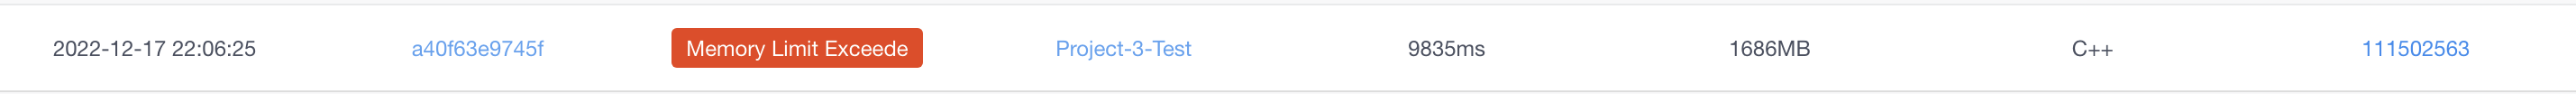
\includegraphics[width=1.1\textwidth]{BottomUp_judge}
		\caption{原始 Bottom up 解法在課程 Online Judge 得執行時間}
		\label{Fig.classOJ1}
	\end{figure}
	
	Bit Operation 版本可以得到很大的提升,執行時間為
	\begin{figure}[hbp]
		\centering
		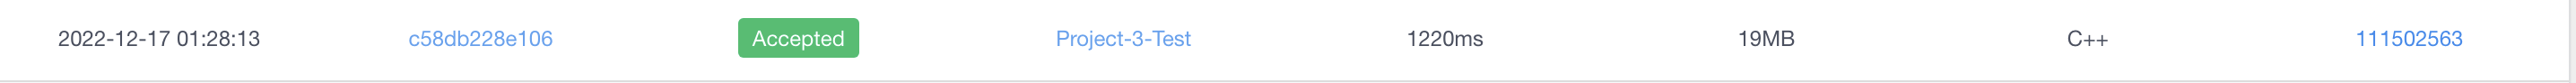
\includegraphics[width=1.1\textwidth]{BitOperation_judge}
		\caption{Bit Operation解法在課程 Online Judge 得執行時間}
		\label{Fig.classOJ2}
	\end{figure}

	Top Down 解法,效果非常好,此時的執行時間已經能夠在 1 秒之內執行完畢了。
	\begin{figure}[hbp]
		\centering
		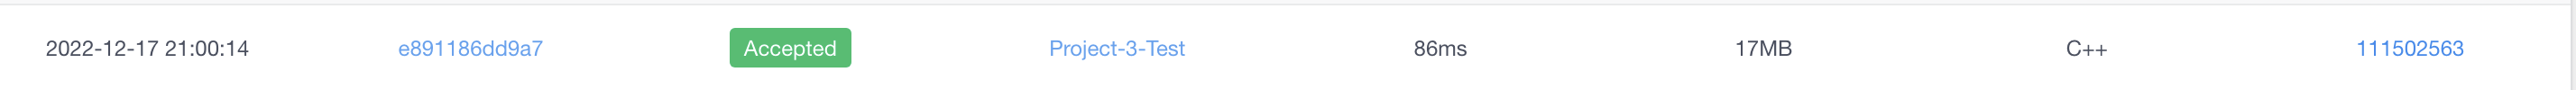
\includegraphics[width=1.1\textwidth]{TopDown_judge}
		\caption{Top Down 解法在課程 Online Judge 得執行時間}
		\label{Fig.classOJ3}
	\end{figure}


	\part{Conclusion \& Reflection}
	
	本篇使用三種解法實作處理 UVA 10482 The candyman can 的問題,在原題目的解法在增加難度後完全不可行,因為空間已經過大了,但觀察遞迴式可以簡單的轉換到 Bit Operation,使用 bitset 可以讓我更輕鬆撰寫程式,不必處理怎麼 32 個包裝的問題,最後使用 Top Down 方法,我們只做需要的部分,在時間上有很大的提升。\\
	
	本次專題讓我知道我對 DP 並不熟,相較於前兩次專題這次專題我面臨更大挑戰,我原本就沒有學過太多的 DP 技巧,只能從遞迴式寫出程式,但這次要我從頭設計 DP 算法解決一個問題,Top Down 的解法真的讓我對 DP 有新的見解,也才知道 Top down 跟 bottom up 的差別。
\end{document}